%% SecureSpeak — Paper 1 — ACM DTRAP submission
%% Compile on Overleaf with the "acmart" template (documentclass below).
%% For initial submission ACM journals use the single-column manuscript mode.
\documentclass[manuscript,screen,review]{acmart}

%% --- Journal identification (DTRAP) -----------------------------------
\acmJournal{DTRAP}
\acmVolume{0}
\acmNumber{0}
\acmArticle{0}
\acmYear{2026}
\acmMonth{7}

%% Remove ACM reference-format block noise while in review (optional).
\settopmatter{printacmref=true}
\setcopyright{none}
\renewcommand\footnotetextcopyrightpermission[1]{}

\usepackage{booktabs}
\usepackage{graphicx}

\begin{document}

\title{SecureSpeak: A Layered Phishing, Smishing, and Malware Defense for Mobile Financial Services in Bangladesh}

\author{Khondokar Sajid}
\authornote{Corresponding author and lead author.}
\affiliation{%
  \institution{North South University}
  \department{Department of Electrical and Computer Engineering}
  \city{Dhaka}
  \country{Bangladesh}}
\email{khsajid3134@gmail.com}

\author{Abdul Alim Rakib}
\affiliation{%
  \institution{North South University}
  \department{Department of Electrical and Computer Engineering}
  \city{Dhaka}
  \country{Bangladesh}}
\email{abdulalimrakib04@gmail.com}

\author{Nova Ahmed}
\affiliation{%
  \institution{North South University}
  \department{Department of Electrical and Computer Engineering}
  \city{Dhaka}
  \country{Bangladesh}}
\email{nova.ahmed@northsouth.edu}

\renewcommand{\shortauthors}{Sajid, Rakib, and Ahmed}

\begin{abstract}
Mobile Financial Services (MFS) such as bKash, Nagad, and Rocket are critical financial infrastructure in Bangladesh, and their users---often elderly, first-time smartphone owners, or low-literacy remittance recipients---are disproportionately exposed to phishing and smishing. A national survey reports that roughly nine percent of MFS users have been defrauded, at an average loss on the order of nine thousand taka. We present SecureSpeak, a layered detection system combining a URL phishing detector, a Bangla/Banglish smishing classifier, and a network-flow anomaly detector behind a lightweight decision layer that produces bilingual, low-literacy warnings. We evaluate every text component under two split protocols and report both. The URL detector reaches 99.19\% accuracy and 0.9976 ROC-AUC under a registered-domain-disjoint split with zero domain overlap, against 99.65\% under a conventional random split; the small gap establishes generalization rather than sibling recognition. The Bangla smishing detector reaches 95.76\% accuracy under a near-duplicate-disjoint split, against 97.84\% under a random split, while its false-negative rate improves from 1.89\% to 1.11\%. The URL detector further transfers to the independent PhiUSIIL corpus with no accuracy loss, reaching 99.61\% on 177{,}933 unseen URLs after removing verbatim overlap, evidence that it has learned generalizable structure. Alongside these system results we report a methodological finding we expect to be broadly useful: the MFS-specific features we engineered produce no measurable accuracy benefit (ablation $-0.0001$, 95\% CI $[-0.0003, +0.0001]$, McNemar $p=0.508$; SHAP ranks 17--21 of 26), and an audit of the evaluation corpora explains why---the phishing corpus contains six MFS-brand URLs in a test set of 29{,}794, and the Bangla SMS benchmark is 56.5\% exact duplicates. MFS-targeted attacks are largely absent from the corpora on which defences against them are evaluated. We report this in full, decline to make claims the data cannot support, and argue that constructing adequate evaluation corpora is a precondition for progress in this area.
\end{abstract}

\begin{CCSXML}
<ccs2012>
<concept>
<concept_id>10002978.10002991.10002995</concept_id>
<concept_desc>Security and privacy~Phishing</concept_desc>
<concept_significance>500</concept_significance>
</concept>
<concept>
<concept_id>10002978.10003029</concept_id>
<concept_desc>Security and privacy~Human and societal aspects of security and privacy</concept_desc>
<concept_significance>300</concept_significance>
</concept>
<concept>
<concept_id>10010147.10010257</concept_id>
<concept_desc>Computing methodologies~Machine learning</concept_desc>
<concept_significance>300</concept_significance>
</concept>
</ccs2012>
\end{CCSXML}

\ccsdesc[500]{Security and privacy~Phishing}
\ccsdesc[300]{Security and privacy~Human and societal aspects of security and privacy}
\ccsdesc[300]{Computing methodologies~Machine learning}

\keywords{phishing detection, mobile financial services, smishing, Bangla NLP, evaluation methodology, dataset quality, data leakage, usable security, Bangladesh}

\maketitle

\section{Introduction}
Mobile Financial Services have transformed financial inclusion in Bangladesh. Platforms such as bKash, Nagad, and Rocket now reach a large share of the adult population and carry everyday wages, remittances, and pensions. This growth has been accompanied by a persistent rise in fraud. A survey by the Policy Research Institute of Bangladesh found that roughly one in ten MFS users---about 9.3 percent---had been the victim of some form of fraud, with an average loss on the order of nine thousand taka, and that fear of fraud is a common reason non-users cite for avoiding MFS entirely~\cite{pri2022}. The users at greatest risk---elderly pensioners, first-time smartphone owners, and rural remittance recipients---are precisely those least equipped to recognize a fraudulent link or a spoofed sender.

The threat is not hypothetical. SikkahBot, an Android malware campaign active since July 2024 and documented by Cyble Research and Intelligence Labs, impersonates official Bangladesh Education Board scholarship portals, intercepts SMS, abuses the Android Accessibility Service to autofill stolen PINs into bKash, Nagad, and Dutch-Bangla Bank apps, and executes offline USSD transactions, while maintaining low detection rates on public scanners~\cite{sikkahbot}. Campaigns of this kind exploit a detection gap, because newly registered domains and repackaged apps evade blacklists and structure-based classifiers, and a comprehension gap, because a warning a low-literacy user cannot read or act upon provides no protection.

This paper reports the design and honest evaluation of SecureSpeak, conducted under two commitments. The first is protocol rigor. Aggregate accuracy on a random split is a weak claim for text classification in this domain: phishing corpora contain many URLs per registered domain, and SMS corpora contain templated messages repeated at scale, so a random split places near-copies of test items into training. We therefore evaluate both text components under grouped, leakage-controlled protocols and report both numbers. The second commitment is that negative results are reported as prominently as positive ones.

That second commitment turned out to matter more than we anticipated. The MFS-specific knowledge features that motivated the system's design produce no measurable accuracy benefit, and rank in the bottom third of the feature set by attribution. Investigating why led to a finding about the evaluation data rather than about our model: the phishing corpus we use, among the most current available, contains six MFS-brand URLs in a held-out set of 29{,}794, and the Bangla SMS benchmark is more than half exact duplicates. The attacks that cost Bangladeshi MFS users an average of nine thousand taka per incident are close to absent from the data the field uses to build defences against them. We consider establishing that fact, with measurements, to be a central methodological contribution of this paper, standing alongside the detection system itself.

\paragraph{Contributions}
\begin{itemize}
\item A URL phishing detector evaluated under a \emph{registered-domain-disjoint} split, reaching 99.19\% accuracy and 0.9976 ROC-AUC with zero domain overlap, against 99.65\% under a random split. The 0.46\% relative gap establishes generalization to unseen domains.
\item A Bangla/Banglish smishing classifier evaluated under a \emph{near-duplicate-disjoint} split, reaching 95.76\% accuracy against 97.84\% under a random split, with false-negative rate improving from 1.89\% to 1.11\% under the stricter protocol.
\item Two convergent \emph{negative results} on the MFS-specific features: a null ablation ($-0.0001$, 95\% CI $[-0.0003, +0.0001]$, $p=0.508$) and bottom-third SHAP attribution (ranks 17--21 of 26) on the model we report.
\item An \emph{audit of both evaluation corpora} that explains those results: 6 MFS-brand URLs in 29{,}794 test URLs, and 56.5\% exact duplication in the 2{,}772-message Bangla SMS benchmark, reducing to 1{,}028 distinct clusters.
\item \emph{Cross-dataset generalization}: the URL detector, trained on StealthPhisher, reaches 99.61\% accuracy and 0.9985 ROC-AUC on 177{,}933 unseen URLs from the independent PhiUSIIL corpus after removing shared URLs, evidence of learned structure rather than corpus-specific artifacts.
\item A \emph{lightweight, interpretable, updatable decision layer} with a bilingual low-literacy warning design, an honest account of the network detector's ceiling on unseen malware families and its domain shift on real Bangladeshi device traffic, and on-device latency and memory measurements.
\end{itemize}

SecureSpeak is thus two contributions in one artifact: a deployable, honestly-evaluated layered detector for a threat that endangers millions of financially vulnerable users, and a measurement result---the near-absence of MFS-targeted attacks from the corpora the field evaluates on---that reframes what ``progress'' on this problem currently means. We regard the second as the more durable: models improve quickly, but a community cannot measure progress against a threat its benchmarks do not contain.

\section{Background and Threat Model}
\subsection{Mobile Financial Services in Bangladesh}
MFS in Bangladesh is not a convenience layer over conventional banking; for a large part of the population it is the primary channel for receiving wages and remittances and for making everyday payments. The survey that reports the fraud rate also records that the majority of surveyed users transact through bKash, with Nagad and Rocket following~\cite{pri2022}. Adoption has outpaced security literacy: many users are first-time smartphone owners, operate on intermittent data connections, and rely on agents. These conditions make brand-impersonating attacks especially effective, because the user's trust in a familiar brand name is itself the attack surface.

\subsection{Threat Model}
We consider an attacker seeking to steal MFS credentials---a PIN or one-time password---or to induce a fraudulent transfer, through three vectors: phishing URLs delivered via SMS or messaging apps; Bangla or Banglish smishing messages creating urgency around an account, a prize, or a disbursement; and malicious applications that generate anomalous network activity once installed. Because a missed attack costs a user money while a false alarm is an annoyance, we treat false-negative rate as the primary cost throughout, and report it for every text component.

\paragraph{Out of scope} SecureSpeak does not address authorized-push-payment fraud, in which a user is socially engineered into willingly sending money and no technical artifact is malicious; insider fraud at the operator or agent level; or SIM-swap attacks. These require organizational or regulatory controls beyond an on-device detector.

\section{System Design}
SecureSpeak is organized as three independent detectors feeding a single decision layer, as shown in Figure~\ref{fig:arch}. The detectors are deliberately heterogeneous---a tree ensemble for URLs, a sentence-embedding classifier for SMS, and a flow-based detector for network traffic---because the three signals have different operating characteristics and different relevance depending on context.

\begin{figure}[t]
\centering
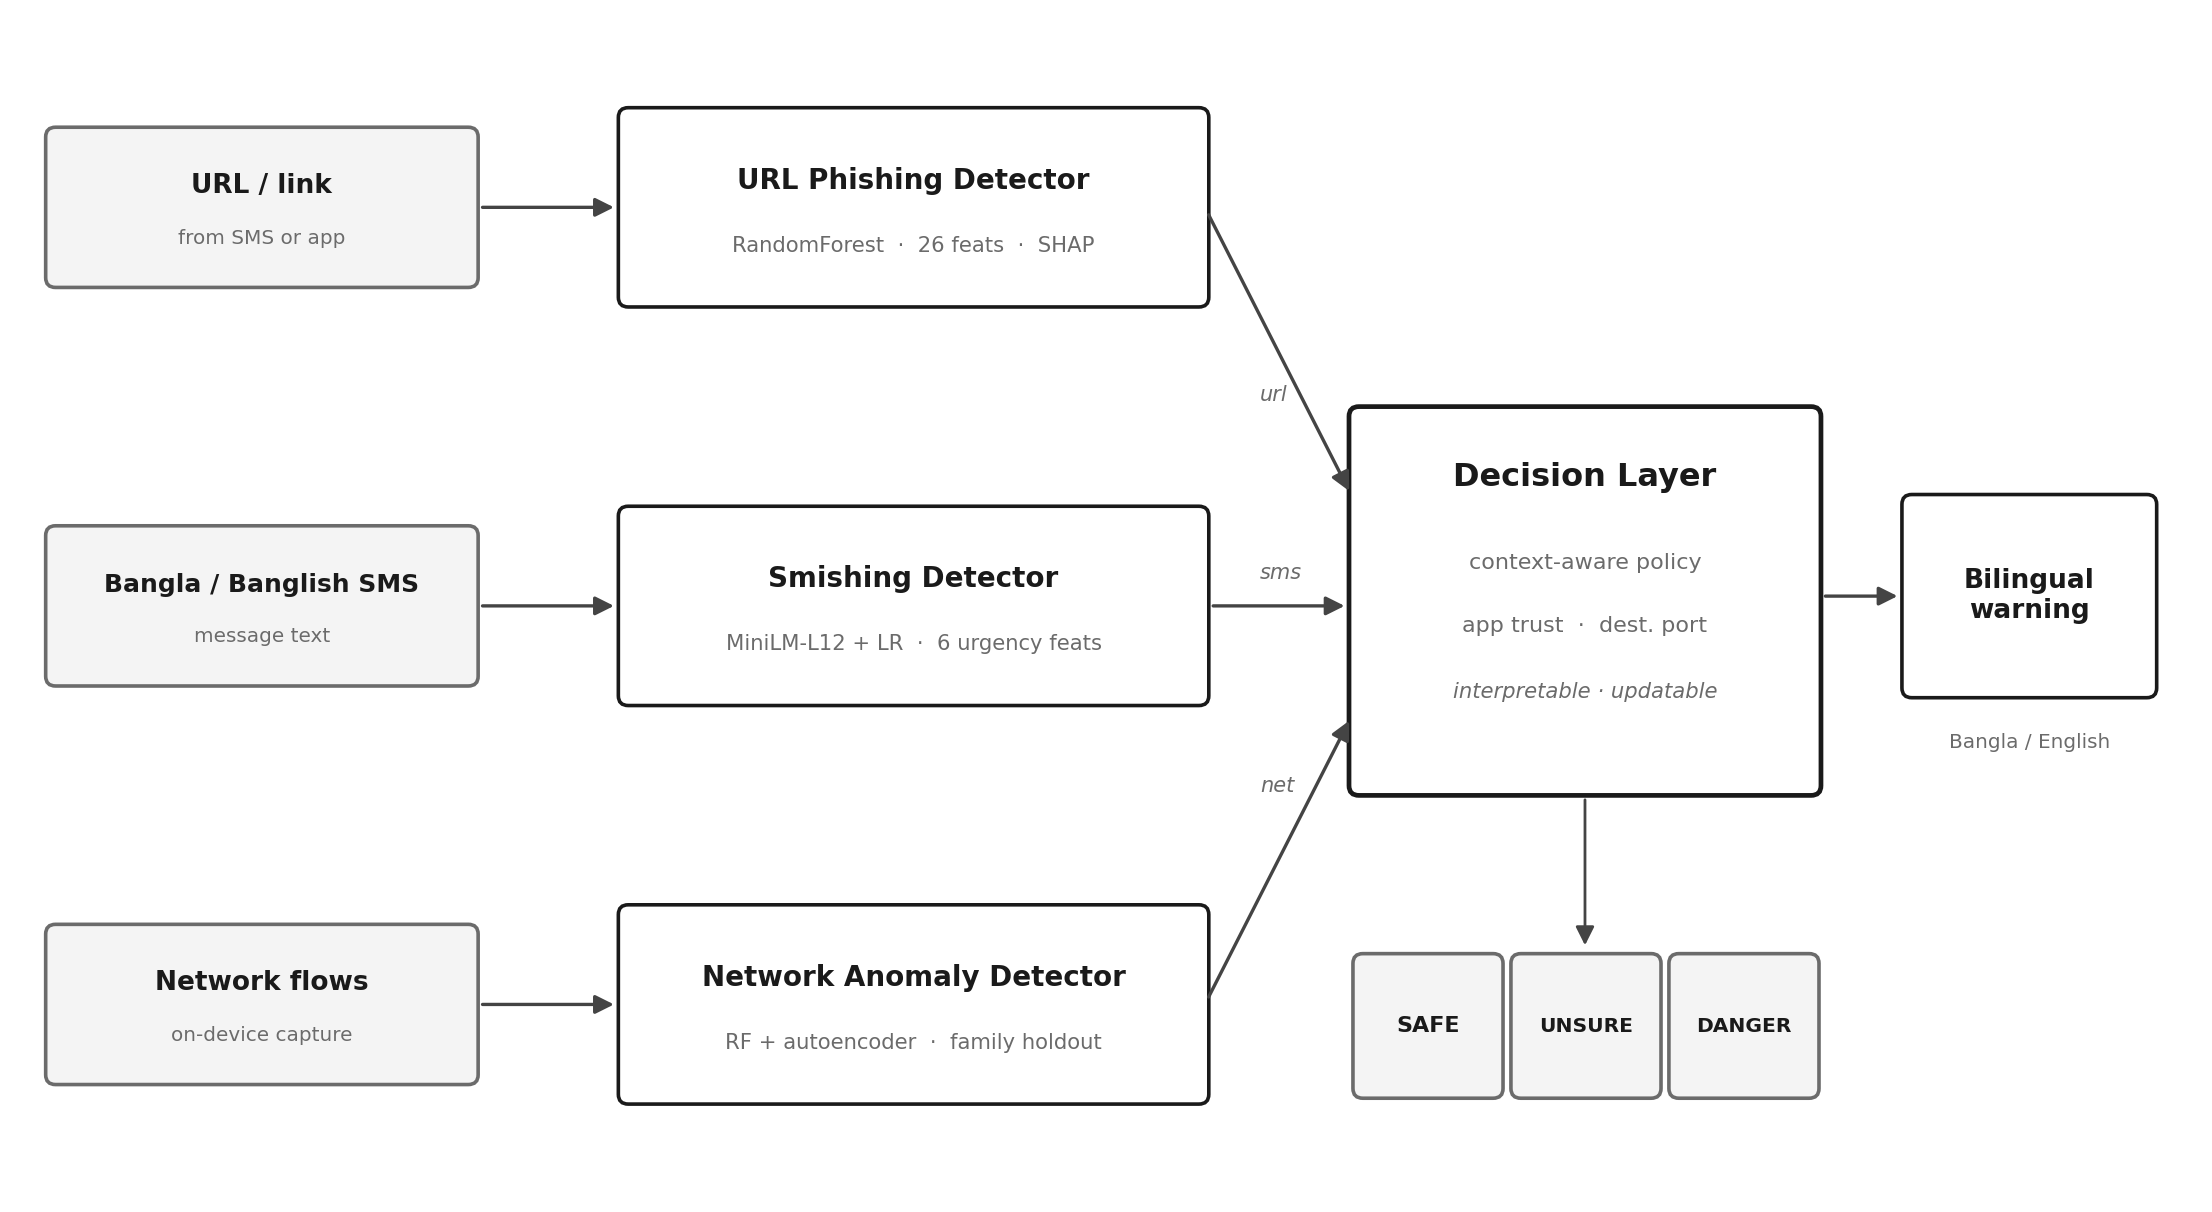
\includegraphics[width=\linewidth]{fig1_architecture.png}
\caption{SecureSpeak architecture. Three detectors feed a context-aware decision layer that emits a three-zone outcome (SAFE / UNSURE / DANGER) and a bilingual, low-literacy warning.}
\label{fig:arch}
\end{figure}

\subsection{URL Phishing Detector}
The URL detector engineers 26 numerical features from each URL string, grouped into lexical structure, domain risk, entropy, Bangladesh-specific signals, and structural patterns. Four features encode MFS domain knowledge: a brand-impersonation count over MFS and global brand tokens appearing in the registrable domain; a financial-keyword density feature calibrated for bKash, Nagad, and Rocket alongside generic banking terms; a free-hosting TLD indicator for the \texttt{.tk/.ml/.ga/.cf/.gq/.pw} cluster; and a broader high-risk TLD indicator. A Random Forest of 300 trees with balanced class weighting is trained on the StealthPhisher 2025 corpus~\cite{stealthphisher}. Standardization is wrapped with the classifier in a single pipeline so normalization statistics are fitted only on training folds. SHAP values are computed with a tree explainer so that the features driving each decision can be passed to the warning generator.

\paragraph{Implementation note} The brand-impersonation feature tests brand tokens against the registrable domain without reference to a whitelist of official MFS domains. It therefore fires on the presence of a brand token in a domain, not on its presence in an unauthorized domain specifically. A whitelist-backed formulation would be stronger, and we treat the current one as a limitation rather than a contribution.

\subsection{Bangla/Banglish Smishing Detector}
The SMS detector embeds each message with \texttt{paraphrase-multilingual-MiniLM-L12-v2}, which produces 384-dimensional sentence embeddings for more than fifty languages including Bangla, at a fraction of the inference cost of a full transformer such as mBERT or BanglaBERT~\cite{reimers2020}. This choice is deliberate: the target devices are mid-range Android phones, and an encoder that cannot run cheaply on such hardware cannot reach the users who need it. The embedding is concatenated with six handcrafted features---URL presence, MFS keyword presence, urgency keyword presence, normalized message length, exclamation density, and digit ratio---giving a 390-dimensional vector classified by logistic regression with the SAGA solver and balanced class weights.

\subsection{Network Anomaly Detector}
The network detector addresses post-click malware---applications that behave normally at install time but generate anomalous traffic afterward. We position it deliberately as a conservative supporting signal rather than a primary defence: the URL and SMS detectors carry the detection load, and the network layer exists to add evidence for untrusted applications without disrupting legitimate local traffic such as bKash, Nagad, WhatsApp, and Facebook. A supervised Random Forest is trained on CICFlowMeter flow records from CICMalAnal2017. To estimate generalization to unseen families rather than within-distribution recognition, we withhold the SCAREWARE family entirely from all training using a family-level physical holdout, enforced by a runtime family-overlap assertion, following stricter protocols advocated for malware classification~\cite{taheri2019,pendlebury2019}. We also evaluated an autoencoder trained only on benign flows as an unsupervised zero-day signal~\cite{sakurada2014}; as Section~\ref{sec:scareware} shows, its separation on the withheld family is near chance, so we retain it only as a reported baseline and do not rely on it in the decision pipeline. In the decision layer, the network score is consulted only for traffic from applications outside the trusted set; for trusted MFS and messaging apps the score is down-weighted, so a domain-shifted or unreliable score cannot by itself raise an alarm on a known-good application.

\subsection{Decision Layer and Bilingual Warnings}
A lightweight decision layer combines detector outputs with two pieces of deployment context---the trust level of the originating application and the destination port---and maps the result to SAFE (silent), DANGER (block with a warning), or UNSURE (protect by default with a recognition-based prompt). The layer is intentionally not a monolithic learned model. It is interpretable per decision, since the outcome traces to specific signals and explicit context rules, and updatable without retraining, since a newly identified malicious port or package name can be added to the rules and immediately extends coverage. Warnings are constructed from rule-based bilingual templates keyed to the top contributing features, so that a flagged link produces a specific, recognition-based message in Bangla and English (for example, ``\bn{this link uses a free .tk domain and contains the word bKash}). We deliberately avoid on-device generative models: an 8-billion-parameter language model cannot run within the memory and latency budget of the low-end Android phones our target users own, and a fixed template that names the triggering feature is both cheaper and more predictable than generated text. We make no quantitative claim for this layer in this paper; its updatability property is argued from construction rather than measured, and a controlled comparison against a learned fusion baseline is identified as ongoing work. The comprehension and protective value of these templated warnings among elderly and low-literacy users is strictly future work and is not evaluated here.

\section{Evaluation}
Every text component is evaluated under two protocols: a conventional random split, and a grouped split in which no group of near-identical items spans the train/test boundary. We report both, along with the group overlap that distinguishes them, so that the contribution of leakage to each headline number is visible rather than assumed away.

\subsection{URL Detector Under Two Split Protocols}
The StealthPhisher 2025 corpus~\cite{stealthphisher} contains 336{,}749 URLs in total; we use the first 150{,}000 (71{,}676 legitimate, 78{,}324 phishing), a 47.8/52.2 class balance identical to that of the full corpus. These 150{,}000 URLs are drawn from 91{,}674 distinct registered domains, an average of 1.64 URLs per domain, with the ten most frequent domains accounting for 19.76\% of all rows. The corpus contains no exact duplicate URLs. Because domains repeat, a random split places siblings of many test URLs into training, and the resulting accuracy partly measures sibling recognition. Table~\ref{tab:splits} reports a stratified random split alongside a split grouped on registered domain.

\begin{table}[t]
\centering
\caption{URL phishing detector under two split protocols. Domain overlap counts registered domains present in both partitions; disjointness is enforced by assertion.}
\label{tab:splits}
\small
\begin{tabular}{lrrrrr}
\toprule
Split protocol & $n$ (test) & Accuracy & ROC-AUC & Recall & FNR \\
\midrule
Random (conventional) & 30{,}000 & 0.9965 & 0.9988 & 0.9954 & 0.0046 \\
\textbf{Domain-disjoint} & \textbf{29{,}794} & \textbf{0.9919} & \textbf{0.9976} & \textbf{0.9853} & \textbf{0.0147} \\
\bottomrule
\end{tabular}
\end{table}

Under the domain-disjoint protocol the detector reaches 99.19\% accuracy and 0.9976 ROC-AUC, against 99.65\% and 0.9988 under a random split: a relative accuracy drop of 0.46\%. We read this small gap as the substantive result. The detector generalizes to registered domains it has never seen, and its headline accuracy is not an artifact of sibling leakage. The cost falls on recall, which declines from 0.9954 to 0.9853 and triples the false-negative rate from 0.46\% to 1.47\%; false-positive rate moves the other way, from 0.22\% to 0.09\%. Since a missed attack is the expensive error in our threat model, the domain-disjoint false-negative rate is the figure a deployment decision should rest on. We report the domain-disjoint result as primary throughout.

\subsection{Ablation of the MFS Knowledge Features}
The system's design premise is that encoding MFS-specific knowledge as engineered features improves detection for the Bangladeshi threat context. We tested this by retraining with all four MFS features removed, on the domain-disjoint split, comparing against the full model on identical test data with a paired bootstrap over 1{,}000 resamples and an exact McNemar test.

\begin{table}[t]
\centering
\caption{Ablation of the four MFS knowledge features (\texttt{brand\_impersonation}, \texttt{financial\_kw}, \texttt{free\_hosting\_tld}, \texttt{high\_risk\_tld}) under the domain-disjoint protocol. $\Delta$ accuracy is computed as full minus ablated; a negative value means the ablated model is marginally more accurate.}
\label{tab:ablation}
\small
\begin{tabular}{lrrrl}
\toprule
Model & Accuracy & Recall & $\Delta$ accuracy (95\% CI) & McNemar $p$ \\
\midrule
Full (26 features) & 0.9919 & 0.9853 & --- & --- \\
Ablated (22 features) & 0.9920 & 0.9854 & $-0.0001\ [-0.0003, +0.0001]$ & 0.508 \\
\bottomrule
\end{tabular}
\end{table}

Removing the MFS features changes accuracy by $-0.0001$, with a confidence interval spanning zero and a McNemar $p$-value of 0.508. There is no measurable accuracy benefit on this corpus.

\subsection{Feature Attribution on the Reported Model}
We computed SHAP attributions with a tree explainer over 2{,}000 sampled test instances from the same domain-disjoint model, to establish which features the reported classifier actually relies on. Table~\ref{tab:shap} gives the leading features and the position of each MFS feature.

\begin{table}[t]
\centering
\caption{SHAP attribution over the domain-disjoint model of Table~\ref{tab:splits} ($n=2{,}000$ sampled test instances). Left: five highest-attribution features. Right: the four MFS knowledge features and their ranks among 26.}
\label{tab:shap}
\small
\begin{tabular}{clr}
\toprule
Rank & Feature & mean $|$SHAP$|$ \\
\midrule
\multicolumn{3}{l}{\emph{Five highest-attribution features}} \\
1 & \texttt{slash\_count} & 0.13571 \\
2 & \texttt{path\_length} & 0.11798 \\
3 & \texttt{has\_https} & 0.05706 \\
4 & \texttt{https\_x\_safe\_tld} & 0.04909 \\
5 & \texttt{path\_segments} & 0.04196 \\
\midrule
\multicolumn{3}{l}{\emph{The four MFS knowledge features}} \\
17 & \texttt{high\_risk\_tld} & 0.00187 \\
18 & \texttt{free\_hosting\_tld} & 0.00096 \\
19 & \texttt{financial\_kw} & 0.00070 \\
21 & \texttt{brand\_impersonation} & 0.00002 \\
\bottomrule
\end{tabular}
\end{table}

The model relies on generic structural properties of the URL string. The four MFS features occupy ranks 17, 18, 19, and 21 of 26, and \texttt{brand\_impersonation} registers a mean absolute attribution of 0.00002, which is effectively zero. The ablation and the attribution therefore agree: on this corpus the MFS features carry no weight. This is not a critique of the feature design. It is a quantitative demonstration that the evaluation corpus does not contain the MFS-specific threats these features were built to catch---a feature cannot influence a decision about an attack that is absent from the data. We note this explicitly because an earlier iteration of this work reported these features among the most influential, a result obtained on a smaller sample under a random split which does not reproduce on the model reported here.

\subsection{Why Both Results Are Null: An Audit of the Evaluation Corpora}
A feature cannot contribute to a decision about an attack that is not present in the test data. We therefore audited both text corpora for the attacks the system targets. Table~\ref{tab:audit} summarizes what we found.

\begin{table}[t]
\centering
\caption{Audit of the two text evaluation corpora. Near-duplicate clusters are formed by normalizing digits and URLs, then merging messages with character $n$-gram cosine similarity above 0.90.}
\label{tab:audit}
\small
\begin{tabular}{llr}
\toprule
Corpus & Property audited & Measurement \\
\midrule
StealthPhisher 2025 & Test URLs containing an MFS brand token & \textbf{6 of 29{,}794 (0.02\%)} \\
(150{,}000 URLs used) & Distinct registered domains & 91{,}674 \\
 & Exact duplicate URLs & 0 \\
BangalaBarta 2024 & Exact duplicate messages & \textbf{1{,}566 of 2{,}772 (56.5\%)} \\
(2{,}772 messages) & Distinct messages after normalization & 1{,}095 \\
 & Distinct near-duplicate clusters & 1{,}028 \\
 & Largest single cluster & 48 identical messages \\
\bottomrule
\end{tabular}
\end{table}

Six of 29{,}794 held-out URLs contain an MFS brand token. That is 0.02\%, too few for any subgroup analysis and far too few to influence an aggregate metric. The MFS features are not ineffective; they are untested, because the attack class they target is effectively absent from the corpus. This holds beyond our system: StealthPhisher 2025 is among the most current large-scale phishing URL corpora available, and it contains almost no examples of the attack that costs Bangladeshi MFS users an average of nine thousand taka per incident. Any detector for this threat, ours included, is presently evaluated on data that does not contain it.

The Bangla SMS benchmark presents a different problem. Of 2{,}772 messages, 1{,}566 are exact duplicates of another message in the corpus, and normalizing digits and URLs leaves 1{,}095 distinct texts. Near-duplicate clustering reduces the corpus to 1{,}028 groups, the largest containing 48 identical copies of a single mobile-operator data-pack advertisement. A corpus of this size and composition supports a narrower range of claims than its nominal message count suggests, and any random split over it distributes members of the same cluster across both partitions.

\subsection{Bangla Smishing Detector Under Two Split Protocols}
We therefore evaluated the smishing detector under a random split and under a split grouped on the near-duplicate clusters of Table~\ref{tab:audit}, so that no cluster spans the boundary.

\begin{table}[t]
\centering
\caption{Bangla/Banglish smishing detector under two split protocols. Cluster overlap counts near-duplicate clusters present in both partitions.}
\label{tab:sms}
\small
\begin{tabular}{lrrrrr}
\toprule
Split protocol & $n$ (test) & Accuracy & ROC-AUC & Recall & FNR \\
\midrule
Random (conventional) & 555 & 0.9784 & 0.9981 & 0.9811 & 0.0189 \\
\textbf{Cluster-disjoint} & \textbf{543} & \textbf{0.9576} & \textbf{0.9800} & \textbf{0.9889} & \textbf{0.0111} \\
\bottomrule
\end{tabular}
\end{table}

Accuracy falls from 97.84\% (95\% CI $[96.58, 98.92]$, $n=555$) to 95.76\% (95\% CI $[94.11, 97.24]$, $n=543$) when near-duplicate clusters are prevented from spanning the split. We apply the same rigor here that we applied to the URL ablation: the two confidence intervals overlap, and an exact McNemar test on the messages present in both test partitions ($n=109$, three discordant predictions) gives $p=1.0$. The point-estimate drop is therefore real but is not statistically distinguishable from noise on a test set this small---an honest limitation of evaluating on a corpus that reduces to roughly a thousand distinct clusters. The detector relies on template memorization to a measurable but statistically modest degree. One effect runs counter to the accuracy figure and matters more under our threat model: the false-negative rate improves under the stricter protocol, from 1.89\% to 1.11\%, with recall rising from 0.9811 to 0.9889. The cluster-disjoint model misses fewer attacks and raises more false alarms. Since a missed attack costs a user money and a false alarm costs them an interruption, the honest protocol produces the operationally preferable model.

The strongest published result on this corpus is that of Tanbhir et al.~\cite{tanbhir2024}, who report 98.47\% using BERT with a character-level CNN and attention, and who constructed the corpus. Their evaluation, like our random-split figure of 97.84\%, is a conventional split and is subject to the same duplication. Our 95.76\% is not a like-for-like comparison against 98.47\% and should not be read as one; the comparable pairing is 97.84\% against 98.47\%. On that basis our result is 0.63 points lower, from a distilled 384-dimensional sentence encoder with logistic regression rather than a BERT-plus-CNN hybrid. For a system whose value depends on running on the phone of an elderly pensioner in a rural district, comparable accuracy at substantially lower inference cost is the operationally meaningful comparison.

\subsection{Network Anomaly Detector}
Table~\ref{tab:net} reports the supervised classifier on the balanced CICMalAnal2017 set with the SCAREWARE family withheld from all training.

\begin{table}[t]
\centering
\caption{Network classifier on CICMalAnal2017 (balanced, SCAREWARE family withheld). Values are single-run point estimates for model selection and are not accompanied by confidence intervals; the selected model is the one carried forward.}
\label{tab:net}
\small
\begin{tabular}{lrr}
\toprule
Model & Test accuracy & ROC-AUC \\
\midrule
\textbf{Random Forest (selected)} & \textbf{0.7984} & \textbf{0.8421} \\
XGBoost & 0.7062 & 0.8105 \\
LightGBM & 0.6765 & 0.7843 \\
\bottomrule
\end{tabular}
\end{table}

The selected Random Forest reaches 79.84\% accuracy and 0.8421 AUC, with a 5-fold cross-validated F1 of $0.8611 \pm 0.0009$ on the training split. This figure must be read against its protocol. Published results on CICMalAnal2017 routinely exceed 95\% accuracy, but those numbers are obtained under random splits that place samples of every malware family in both the training and test partitions; they measure a model's ability to recognize families it has already seen, not its ability to catch new ones. We deliberately reject that protocol. By physically withholding the entire SCAREWARE family from training, we force the detector to confront a malware class it has never encountered, which is the situation that matters operationally, since the threats an on-device detector meets in deployment are precisely the ones absent from its training data. Under this stricter and, we argue, more meaningful evaluation, 79.84\% is a conservative but honest number; a 95\% figure on this corpus should be treated as evidence of family leakage rather than of zero-day capability. This is the figure a deployment engineer should use for capacity planning, not the leaky within-distribution score. \label{sec:scareware}We also quantified the reconstruction-error detector on the withheld SCAREWARE family directly. Trained only on benign flows and evaluated on its ability to separate benign traffic from unseen scareware, it achieves an ROC-AUC of just 0.513---statistically indistinguishable from chance---recovering 5.8\% of scareware flows at a 5\% benign false-positive rate and 11.4\% at 10\%. This near-random separation is not a defect in the detector but a property of the threat: scareware traffic mimics ordinary HTTPS and is nearly indistinguishable from benign flows on flow statistics alone. It is a real and instructive ceiling, and quantifying it as an AUC rather than a single operating point makes the limitation explicit: pure flow-based anomaly detection cannot, by itself, catch a genuinely novel malware family that behaves like normal encrypted traffic. We therefore treat the network signal as a deliberately conservative supporting input to the decision layer rather than a standalone authority, and we consider an honest 79.84\% under family holdout more useful to a practitioner than an inflated within-distribution score.

\subsection{Domain Shift on Real Bangladeshi Device Traffic}
Applying the supervised detector, trained on the Western CICMalAnal2017 corpus, to 52{,}118 flows captured with PCAPdroid from six Android devices belonging to the authors, in ordinary daily use in Bangladesh, exposes a domain-shift problem. The feature distributions of legitimate local traffic---bKash, Facebook, WhatsApp, local news applications---differ from the training corpus's benign class, and the two capture pipelines do not expose an identically aligned feature space. Raw supervised scores consequently do not transfer in a way that supports a real-world false-positive claim, and we report no false-positive rate on this set: a score that is constant or uninterpretable across real flows would be meaningless however favourable it appeared. We treat this as a limitation with two mitigations. First, the decision layer down-weights network evidence for trusted applications, so a domain-shifted score cannot by itself raise an alarm on a known-good app. This mitigation covers most traffic in practice: classifying our 52{,}118 real flows by originating application, 67.8\% (35{,}355 flows) come from trusted applications---MFS apps, major messaging platforms, and system services---for which the network score is down-weighted, leaving 32.2\% from untrusted or unknown applications (led by web browsers, TikTok, and assorted utilities) where the score is actually consulted. The domain-shift problem is therefore confined to roughly a third of real traffic rather than applying to all of it. Second, feature-space alignment between the capture tools, with on-device fine-tuning, is the primary future-work item for this component. We report the 67.8\% trusted fraction as a measured property of real device usage, not an assumption; it bounds how often the network layer is even active, and it is the honest complement to the family-holdout and SCAREWARE results above.

\subsection{On-Device Latency and Memory}
We measured the pipeline's per-item cost on a single CPU core (Intel Xeon, Google Colab, no GPU, single-threaded) as a proxy for mid-range Android hardware. A server Xeon core is likely faster per-thread than a mid-range ARM core, so these figures are best read as a lower bound on real-device latency rather than a conservative upper bound; we report them to establish order of magnitude. We score one item at a time rather than in batches, because a phone processes a single link or message as it arrives. End to end, including feature engineering, the URL detector scores a link in 85\,ms on average (95th percentile 150\,ms), and the smishing detector classifies a message in 44\,ms on average (95th percentile 67\,ms), the latter dominated by the MiniLM forward pass. Both are well within interactive latency for a per-item check, and feature engineering itself is negligible at well under a millisecond per URL.

Memory is the real deployment constraint, and we report it plainly rather than minimizing it. The two deployable models are the URL Random Forest at 42\,MB and the multilingual sentence encoder at 471\,MB in full precision; the rule-based warning templates and the decision-layer logic add negligible footprint, and no generative model is deployed. The encoder dominates and is large for a low-end device, but int8 quantization reduces it roughly fourfold to about 118\,MB, bringing the entire deployable pipeline to under 160\,MB, within the budget of a mid-range Android phone. On-device distillation of the encoder is a natural further step. These figures establish that the pipeline is viable on device for the latency-sensitive URL and SMS checks, while identifying the encoder's size as the principal engineering constraint a production deployment must address. Figures are single-core CPU measurements and are indicative rather than exact for any specific handset.

\subsection{Cross-Dataset Transfer}
A detector evaluated on a single corpus, however carefully split, leaves open whether it has learned the phenomenon or the corpus. We therefore tested the StealthPhisher-trained URL model, unchanged, on the independent PhiUSIIL corpus~\cite{phiusiil} of 235{,}795 URLs (134{,}850 legitimate, 100{,}945 phishing), built by a different group from different sources. Because all 26 features are computed from the URL string alone, no retraining or adaptation is required.

An initial run scored 99.66\% accuracy on PhiUSIIL, marginally above the in-corpus figure. We treated a cross-corpus result at or above the in-corpus number as a warning sign rather than a success, and audited the two corpora for shared URLs. They overlap substantially: 57{,}695 distinct PhiUSIIL URLs (24.5\% of the corpus) appear verbatim in the StealthPhisher training set, and 48{,}653 PhiUSIIL registered domains (27.7\%) are also present in training. The inflated figure was therefore partly memorization. We then discarded every PhiUSIIL record whose URL appears anywhere in training and re-evaluated on what remained: 177{,}933 records with genuinely unseen URLs, on which the model reaches \textbf{99.61\% accuracy and 0.9985 ROC-AUC} (Table~\ref{tab:transfer}). This is the figure we report. (The evaluated counts are record counts; because PhiUSIIL contains some repeated URLs, they are not a direct subtraction of the distinct-URL overlap from the corpus size.)

\begin{table}[t]
\centering
\caption{Cross-dataset transfer of the URL detector, trained on StealthPhisher and evaluated on PhiUSIIL. The final row excludes every PhiUSIIL record whose URL appears verbatim in the training corpus and is the figure we report; counts are records, and PhiUSIIL contains some repeated URLs.}
\label{tab:transfer}
\small
\begin{tabular}{lrrr}
\toprule
Evaluation & $n$ & Accuracy & ROC-AUC \\
\midrule
In-corpus (StealthPhisher, domain-disjoint) & 29{,}794 & 0.9919 & 0.9976 \\
Cross-corpus (PhiUSIIL, all) & 235{,}795 & 0.9966 & 0.9987 \\
\textbf{Cross-corpus (PhiUSIIL, shared URLs removed)} & \textbf{177{,}933} & \textbf{0.9961} & \textbf{0.9985} \\
\bottomrule
\end{tabular}
\end{table}

That the model transfers to an independent corpus with almost no drop from its in-corpus accuracy is evidence that the URL detector has learned generalizable structure rather than corpus-specific artifacts. We note the episode also illustrates the paper's methodological theme: a favourable number that is not audited for overlap can mislead, and the overlap here was large enough to matter.

\section{Discussion}
\subsection{What the Negative Results Mean}
Three measurements converge. The MFS knowledge features produce no accuracy benefit; they rank in the bottom third by attribution, with \texttt{brand\_impersonation} effectively unused; and the corpus on which both were measured contains six MFS-brand URLs in 29{,}794. The third explains the first two. Together they say something we did not set out to demonstrate: this class of attack cannot currently be evaluated, because the data required to evaluate it does not exist in the public corpora the field relies on.

The available alternative was to report the SHAP attribution from an earlier smaller run, in which these features did appear prominent, and let a reader infer benefit. We think that would have been an unsupported claim twice over: attribution describes what a model does with the features it has rather than whether performance degrades without them, and the earlier attribution does not reproduce on the model whose accuracy we report. Stating this costs the paper a claim and gains it a finding.

\subsection{The Interpretability Argument, Stated Precisely}
An earlier framing of this work held that the MFS features earn their place through interpretability even without an accuracy benefit: named, semantically meaningful features with per-decision attribution are what allow a warning to say that a link uses a free \texttt{.tk} domain and contains an MFS brand token, rather than issuing a generic alert. We still regard that as the right architectural argument, and it is why the system uses engineered features with SHAP rather than a learned character-level representation that could not produce such an explanation at all. It must, however, be stated with the limitation attached. On this corpus the mechanism is present but unexercised: a feature with mean absolute attribution of 0.00002 does not enter a top-contributor explanation for any decision, because the inputs that would activate it are almost never seen. We can show the architecture supports specific bilingual warnings; we cannot yet show it produces them for MFS attacks, and we make no claim that it does.

\subsection{Limitations}
\begin{itemize}
\item The MFS knowledge features are unvalidated for both detection benefit and explanation value. No public corpus contains enough MFS-targeted phishing to test either property.
\item The brand-impersonation feature checks brand tokens against the registrable domain without an official-domain whitelist, so it does not distinguish authorized from unauthorized use of a brand name.
\item The Bangla corpus reduces to 1{,}028 distinct near-duplicate clusters, which bounds the strength of any claim drawn from it, including ours.
\item The network detector faces domain shift and a feature-space mismatch on real device traffic, and pure flow statistics have a demonstrated ceiling on unseen malware families.
\item The decision layer's updatability is argued from construction and not measured.
\item All evaluation is on collected and public data. The comprehension and protective value of the bilingual warnings has not been measured with users, and no claim of warning effectiveness is made anywhere in this paper.
\end{itemize}

\subsection{Ongoing and Future Work}
The corpus gap is the first priority, and the item we would most encourage others to treat as shared infrastructure. We are assembling a dedicated MFS-brand phishing URL set from threat feeds, reported fraud SMS, and operator disclosures, sufficient to support a subgroup evaluation of the MFS features, an attribution analysis on decisions where those features are actually active, and a dedicated knowledge-based brand-impersonation layer using an official-domain whitelist, brand-token detection in unauthorized domains, and edit-distance lookalike matching. The second priority is a user study with elderly, low-literacy, and first-time MFS users, evaluating whether the bilingual warnings are understood and acted upon; that is the appropriate venue for any claim about warning effectiveness. Remaining items include a controlled evaluation of the decision layer's update-without-retraining property against a learned fusion baseline, feature-space alignment and on-device fine-tuning for the network detector, and cross-dataset transfer for the URL detector.

\section{Related Work}
URL phishing detection has moved from hand-engineered features on the 2012 UCI corpus~\cite{mohammad2014}, through character-level neural models that trade interpretability for raw performance~\cite{sahingoz2019}, to recent work on current corpora such as StealthPhisher 2025~\cite{stealthphisher}. Our methodological position follows the evaluation-integrity literature: Pendlebury et al.~\cite{pendlebury2019} show that random splits systematically overestimate malware classifier performance and argue for temporal and family-aware protocols, and Taheri et al.~\cite{taheri2019} apply family-level classification to network flows. We apply the same reasoning to URL classification through registered-domain-disjoint splitting and to SMS classification through near-duplicate-cluster-disjoint splitting, and use SHAP~\cite{lundberg2017} for per-decision attribution.

For Bangla SMS, work has progressed from classical classifiers on promotional-spam corpora~\cite{khan2023} to transformer-based approaches~\cite{foysal2025}, at inference costs that preclude on-device deployment. Efficient multilingual sentence encoders produced through knowledge distillation~\cite{reimers2020} make cheap cross-lingual embedding possible, which SecureSpeak exploits. The most directly comparable work is Tanbhir et al.~\cite{tanbhir2024}, who introduce the BangalaBarta corpus~\cite{bangalabarta} and report 98.47\% with a BERT and character-level CNN hybrid; a companion line of work applies BERT-XGBoost with explainable AI to the same corpus~\cite{nirapodbarta}. Khushbu et al.~\cite{khushbu2024} address MFS-specific text fraud with a CNN-LSTM-BiLSTM model on a smaller Bengali corpus. SecureSpeak extends beyond SMS to URLs and network traffic and couples detection with an actionable warning layer.

Network-level Android malware detection has been studied on the CICMalAnal2017 and CICMalDroid2020 families~\cite{lashkari2018,mahdavifar2020}, where random-split evaluation leaks family knowledge and overstates zero-day performance. Reconstruction-based anomaly detection~\cite{sakurada2014} and intrusion datasets such as UNSW-NB15~\cite{moustafa2015} inform the zero-day component, and Isolation Forest~\cite{liu2008} remains a standard unsupervised baseline. Across all of these our position is to treat each signal as one contributor to an interpretable, updatable decision rather than to claim a single dominant model.

\section{Conclusion}
SecureSpeak is a layered detection system built for the Bangladeshi MFS threat context. Its URL detector reaches 99.19\% accuracy and 0.9976 ROC-AUC under a registered-domain-disjoint split with zero domain overlap, a protocol that establishes generalization rather than sibling recognition. Its Bangla smishing detector reaches 95.76\% under a near-duplicate-disjoint split, and improves its false-negative rate to 1.11\% under that stricter protocol. Its network detector is reported honestly, including a family-holdout figure that is not comparable to published random-split results and a domain-shift limitation on real device traffic that we decline to convert into a favourable-looking number.

Beyond the per-component results, the URL detector transfers to the independent PhiUSIIL corpus with essentially no accuracy loss (99.61\% on 177{,}933 unseen URLs after overlap removal), evidence that it has learned generalizable structure rather than corpus-specific artifacts. The system, in short, works and generalizes. Alongside this, the paper contributes a methodological finding we expect to be widely useful: the MFS-specific features that motivated the design produce no measurable accuracy benefit and rank in the bottom third of the feature set by attribution, and the reason is visible in the data: the phishing corpus contains six MFS-brand URLs in a test set of nearly thirty thousand, and the Bangla SMS benchmark is more than half exact duplicates. The threat that costs Bangladeshi MFS users an average of nine thousand taka per incident is close to absent from the data used to build defences against it. We therefore issue a specific call to the community: the construction of an open, deduplicated, MFS-targeted phishing and smishing corpus is the single highest-leverage contribution the field can now make, and it is a precondition for any credible claim of progress on this threat. Until such a corpus exists, honest evaluation means reporting what current data can and cannot establish---which is what we have tried to do here, weakening our own headline numbers wherever the data did not support them. We would rather publish a defensible measurement than an impressive claim.

\section{Reproducibility}
Every quantitative result in this paper is reproducible from scripted notebooks that regenerate each table in Section~\ref{tab:splits}--\ref{tab:transfer} directly from the public raw corpora. This covers both split protocols, the feature ablation with its bootstrap confidence interval and McNemar test, the SHAP attribution on the reported model, the corpus audits, the cross-dataset transfer with its overlap-removal step, and the on-device latency and memory measurements. Group disjointness is enforced by runtime assertion in the URL and SMS pipelines, and the family-overlap guarantee for the network detector is asserted rather than assumed, so that a run violating any of these constraints halts rather than reporting a leaked number. Random seeds are fixed at 42 throughout. Upon acceptance we will publicly release the complete code, the 26-feature URL extractor, the SMS near-duplicate clustering procedure, the trained model artifacts, and the exact scripts that produce every table and figure, so that an independent reader can reproduce the paper end to end from the public datasets.

\begin{acks}
The authors thank the Department of Electrical and Computer Engineering at North South University. Network traffic was captured on the authors' own devices; no external human subjects were involved in this study.
\end{acks}

\bibliographystyle{ACM-Reference-Format}
\begin{thebibliography}{99}

\bibitem{pri2022} Policy Research Institute of Bangladesh (A. Rahman and A. Rede). 2022. \emph{The State of DFS Consumer Protection in Bangladesh}. Technical Report.

\bibitem{sikkahbot} Cyble Research and Intelligence Labs (CRIL). 2025. \emph{SikkahBot: An Android Malware Campaign Targeting Students and Mobile Financial Services Users in Bangladesh}. Threat Intelligence Report. Campaign active since July 2024.

\bibitem{khushbu2024} S. A. Khushbu, F. T. Jaigirdar, A. Anwar, and Ohidujjaman. 2024. Be Aware of Your Text Messages: Fraud Attempts Identification Based on Semantic Sequential Learning for Financial Transactions through Mobile Services in Bangladesh.

\bibitem{mohammad2014} R. M. Mohammad, F. Thabtah, and L. McCluskey. 2014. Predicting phishing websites based on self-structuring neural network. \emph{Neural Computing and Applications} 25, 2 (2014), 443--458.

\bibitem{sahingoz2019} O. K. Sahingoz, E. Buber, O. Demir, and B. Diri. 2019. Machine learning based phishing detection from URLs. \emph{Expert Systems with Applications} 117 (2019), 345--357.

\bibitem{stealthphisher} T. Jha, H. Goswami, C. Solanki, D. Nagal, V. Yadav, and A. Prasad. 2025. \emph{StealthPhisher: A Phishing Attack Dataset}. Mendeley Data, V1. DOI:10.17632/m2479kmybx.1.

\bibitem{khan2023} F. Khan, R. Mustafa, F. Tasnim, T. Mahmud, M. S. Hossain, and K. Andersson. 2023. Exploring BERT and ELMo for Bangla Spam SMS Dataset Creation and Detection. In \emph{Proc. 26th Int. Conf. on Computer and Information Technology (ICCIT)}.

\bibitem{foysal2025} M. M. R. Foysal and M. S. Rahman. 2025. Bangla SMS Spam Classification Using LLMs: Evaluating the Performance of BanglaBERT and XLM-RoBERTa.

\bibitem{reimers2020} N. Reimers and I. Gurevych. 2020. Making Monolingual Sentence Embeddings Multilingual using Knowledge Distillation. In \emph{Proc. EMNLP}.

\bibitem{lashkari2018} A. H. Lashkari, A. F. A. Kadir, L. Taheri, and A. A. Ghorbani. 2018. Toward developing a systematic approach to generate benchmark Android malware datasets and classification. In \emph{Proc. Int. Carnahan Conf. on Security Technology (ICCST)}.

\bibitem{mahdavifar2020} S. Mahdavifar, A. F. A. Kadir, R. Mahdikhani, H. Ghorbani, and A. A. Ghorbani. 2020. Dynamic Android malware category classification using semi-supervised deep learning. In \emph{Proc. IEEE DASC}.

\bibitem{taheri2019} L. Taheri, A. F. A. Kadir, and A. H. Lashkari. 2019. Extensible Android Malware Detection and Family Classification Using Network-Flows and API-Calls. In \emph{Proc. Int. Carnahan Conf. on Security Technology (ICCST)}.

\bibitem{pendlebury2019} F. Pendlebury, F. Pierazzi, R. Jordaney, J. Kinder, and L. Cavallaro. 2019. TESSERACT: Eliminating experimental bias in malware classification across space and time. In \emph{Proc. USENIX Security Symposium}.

\bibitem{sakurada2014} M. Sakurada and T. Yairi. 2014. Anomaly detection using autoencoders with nonlinear dimensionality reduction. In \emph{Proc. MLSDA Workshop}.

\bibitem{moustafa2015} N. Moustafa and J. Slay. 2015. UNSW-NB15: a comprehensive data set for network intrusion detection systems. In \emph{Proc. MilCIS}.

\bibitem{liu2008} F. T. Liu, K. M. Ting, and Z.-H. Zhou. 2008. Isolation Forest. In \emph{Proc. IEEE Int. Conf. on Data Mining (ICDM)}.

\bibitem{lundberg2017} S. M. Lundberg and S.-I. Lee. 2017. A Unified Approach to Interpreting Model Predictions. In \emph{Proc. NeurIPS}.

\bibitem{bangalabarta} M. F. Shahriyar and G. Tanbhir. 2025. \emph{BangalaBarta: A Spam/Smishing SMS Dataset Bangla}. Mendeley Data, V2. DOI:10.17632/jfkfbw3gzh.2.

\bibitem{tanbhir2024} G. Tanbhir, M. F. Shahriyar, K. Shahed, A. M. R. Chy, and M. Al Adnan. 2024. Hybrid Machine Learning Model for Detecting Bangla Smishing Text Using BERT and Character-Level CNN. In \emph{Proc. 13th Int. Conf. on Electrical and Computer Engineering (ICECE)}. IEEE, 57--62.

\bibitem{nirapodbarta} J. Talukder, G. Tanbhir, M. F. Shahriyar, and G. S. Hossain. 2025. NirapodBarta: A Hybrid BERT-XGBoost Model for Multiclass Bangla Smishing Detection with Explainable AI. In \emph{Proc. 16th Int. Conf. on Computing Communication and Networking Technologies (ICCCNT)}.


\bibitem{phiusiil} A. Prasad and S. Chandra. 2024. PhiUSIIL: A diverse security profile empowered phishing URL detection framework based on similarity index and incremental learning. \emph{Computers \& Security} 136 (2024), 103545. DOI:10.1016/j.cose.2023.103545. Dataset: UCI Machine Learning Repository, id 967.

\end{thebibliography}

\end{document}
